\chapter{Modeling} \label{ch:modeling}

This chapter is concerned with the mathematical model of the wheeled robotic vehicle and will serve as a pre-requisite for the later implemented feedback control algorithm. 
The dynamics part, describing the motor model, will be used in the cruise control derivation. Subsequently the kinematics model, which treats the robot as a point entity, will be used in the estimation for position control.

\section{Differential Drive} \label{kin_model} 

Differential drive steering, a popular choice in mobile robots, is a design where two wheels on a same axle are controlled independently. It may or may not include a castor wheel, however this paper addresses the latter. Depending on the relative rotation of each wheel, the robot could be steered in a desired manner. For the sake of clarity, several basic cases of interest are presented along with the equations describing the linear and angular velocity of the vehicle. 

\begin{align}
v = \frac{Rw_r + Rw_l}{2} \label{eq1} \\
W = \frac{Rw_r - Rw_l}{l} \label{eq2} 
\end{align}

Equation \ref{eq1} describes the linear speed of the robotic vehicle, with respect to the angular speeds of each wheels (\textbf{$w_r$}) and (\textbf{$w_l$}) and the wheel radius (\textbf{R}), while \ref{eq2} describes the angular speed of the robot, with \textbf{l} being the axle length between the wheels. 
The equation could be rewritten in matrix form as:

\[  	
\begin{bmatrix}
	v \\
	\omega	
\end{bmatrix} 
=
\begin{bmatrix} 
	\frac{R}{2} & \frac{R}{2} \\
	\frac{R}{l} & \frac{-R}{l} 
\end{bmatrix}
\begin{bmatrix}
	\omega_r \\
	\omega_l
\end{bmatrix} \label{eq3} 	
\] 

Analysis of the above equation leads to the consideration of three cases where certain behaviour is to be expected.

\begin{itemize} \label{list_v}

\item $\boldsymbol{v_r = v_l}$ \\ In this case scenario, both wheels have the same speed. The robot's speed from equation \ref{eq13} is simply equal to the individual speed of each of wheel. On the other hand, the angular speed from equation \ref{eq14} becomes 0, and the turning radius infinite. The robot is expected to perform straight linear motion.

\item $\boldsymbol{v_r = 0}$ or $\boldsymbol{v_l = 0}$ \\ In this case scenario, the turning radius becomes $\frac{l}{2}$. The robot is expected to perform rotation either about the right or the left wheel, with the center of rotation being the zero velocity wheel. 

\item $\boldsymbol{v_l = -v_r}$ \\ In this case scenario, the turning radius and the linear speed become 0, while the angular speed is doubled. The robot is expected to perform rotation about it's midpoint, or simply put in-place rotation.

\end{itemize}

\subsection{Non-holonomic constraints} 

A robot, using the differential drive steering design, has restricted local movements, while having no restrictions in global motion. \todo{Reference) That is similar to the restrictions on a car, where it is not possible to slide into a parallel position with respect to the current one. Nevertheless, the vehicle can still manoeuvre into the desired position, similar to parallel parking. 

If we consider \todo{insert vehicle figure} we can define the non-holonomic constraints of a differential drive vehicle as: 

\begin{equation} \label{eq4}
\dot{x}sin(\theta) - \dot{y}cos(\theta) = 0
\end{equation}

As observed from equation \ref{eq4} and pictured by \todo{insert fig ref}, the robot can not have speed perpendicular to the sagittal axis. The equation can be further rewritten as:

\begin{equation} \label{eq5} 
\tan{\theta} = \frac{\dot{y}}{\dot{x}} = \frac{dy}{dx}
\end{equation} 

\section{Kinematics} 

The kinematic model, similar to most rigid vehicles travelling on a two-dimensional plane, is of three degrees of freedom. From fig \todo{ref to xy figure}, we can identify \textbf{x} and \textbf{y} as the coordinates for the center of mass of the robot and \textbf{$\theta$} as the angle with respect to the x axis. From the constraints of the vehicle, the equations concerning the kinematic model are derived as:

\begin{align}
\dot{x} = vcos(\theta) \nonumber \\
\dot{y} = vsin(\theta) \label{eq19} \\
\dot{\theta} = \omega  \nonumber 
\end{align}

Where \textbf{v} is the linear and $\textbf{\omega}$ is the angular speed of the vehicle.
The equations could further be represented in matrix form.

\( 	
\begin{bmatrix}
	\dot{x} \\
	\dot{y} \\
	\dot{\theta} \\ 
\end{bmatrix} 
=
\begin{bmatrix} 
	\cos{\theta} & 0 \\
	\sin{\theta} & 0 \\
	0     		 & 1  
\end{bmatrix}
\begin{bmatrix}
	v \\
	\omega
\end{bmatrix} \label{eq3} 	
\)


%The relation between the linear speed and the angular speed of the robot is similar to equation \ref{eq12}.

%\begin{equation} \label{eq15} 
%v = WD
%\end{equation}

%Where D is the turning radius, from the midpoint of the wheels to the ICC. Solving for the turning radius, yields:

%\begin{align}
%D = \frac{v}{W} \label{eq16} \\
%= \frac{l}{2}\frac{v_r + v_l}{v_r - v_l} \nonumber
%\end{align}

\section{Dynamics} \label{dc_math}

\begin{table}[h]
\centering
\begin{tabular}{cccll}
\hline
Parameter                   & Description                               & Unit				 &  &  \\ \hline
\multicolumn{1}{|c|}{K}     & \multicolumn{1}{c|}{Motor constant}       & \multicolumn{1}{c|}{ V/(rad/s)  Nm/amp} &  &  \\ \cline{1-3}
\multicolumn{1}{|c|}{R}     & \multicolumn{1}{c|}{Armature resistance}  & \multicolumn{1}{c|}{$\Omega$}            &  &  \\ \cline{1-3}
\multicolumn{1}{|c|}{L}     & \multicolumn{1}{c|}{Armature inductance}  & \multicolumn{1}{c|}{H}                    &  &  \\ \cline{1-3}
\multicolumn{1}{|c|}{$b_r$} & \multicolumn{1}{c|}{Rotor damping}        & \multicolumn{1}{c|}{Nms}                   &  &  \\ \cline{1-3}
\multicolumn{1}{|c|}{$J_w$} & \multicolumn{1}{c|}{Load inertia} & \multicolumn{1}{c|}{$KgM^2$}        &  &  \\ \cline{1-3}
\multicolumn{1}{l}{}        & \multicolumn{1}{l}{}                      & \multicolumn{1}{l}{}                          &  &  \\ \hline
\end{tabular}
\caption{Motor parameters}
\label{my-label}
\end{table}

\begin{figure}[h] %change image
\centering
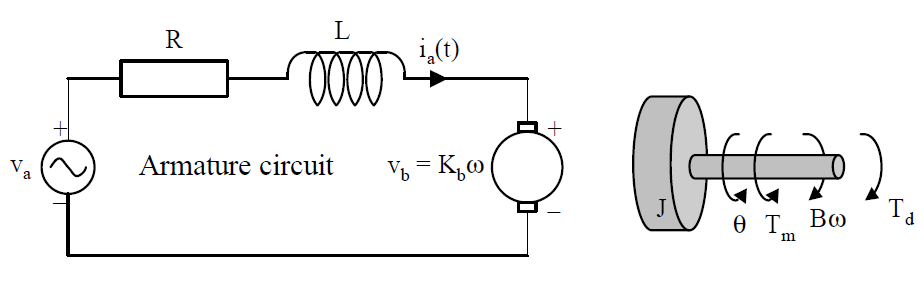
\includegraphics[width = 0.7\textwidth]{Motor_curcuit}
\caption{Electrical circuit and free-body diagram of DC motor \cite{FBD}}
\label{fig::motor_curcuit}
\end{figure} 

In this section the equations used in the dynamics model of the motor are derived and described.

A DC motor produces mechanical torque applied to the shaft($\boldsymbol{T_e}$) linearly proportional to the armature current, the magnetic field and a torque constant($\boldsymbol{K_t}$). Assuming constant magnetic field, the produced torque is proportional to the torque constant($\boldsymbol{K_t}$) and the armature current(\textbf{I}).( Equation \ref{eq1})Furthermore, the back Emf (electromotive force)($E_b$) is equal to the angular velocity($\omega$) of the shaft multiplied with the Back emf constant($K_b$).(Equation \ref{eq2}) \\

\begin{align}  
T_e = IK_t \label{eq1}\\
E_b = \omega K_b \label{eq2}
\end{align}

Because the two constants $K_t$ and $K_b$ are equal in SI units, in further equations and simulations they will be denoted only as a motor constant $K$.

%VERIFY AND MODIFY

\begin{equation} \label{eq3}
K_t = K_b = K
\end{equation} 

Furthermore, from figure \ref{fig::motor_curcuit}, using Kirchhoff's voltage law, we can derive the equations governing the electrical part of the DC motor, where the applied voltage (\textbf{V}) is proportional to the voltage drop through the armature resistance(\textbf{R}) and inductance(\textbf{L}), and the back electromotive voltage($\boldsymbol{E_b}$). \ref{eq4}

\begin{equation} \label{eq4}
V = RI + L\frac{dI}{dt} + E_b
\end{equation} 

The mechanical part of the DC motor(mechanical part of figure \ref{fig::motor_curcuit}) is derived from the equations, where the mechanical torque($\boldsymbol{T_m}$) is the difference between the electromagnetic torque($\boldsymbol{T_e}$) and the rotational losses ($\boldsymbol{T_b}$). \ref{eq5}

\begin{equation} \label{eq5} 
T_m = T_e - T_b
\end{equation} 

Using Newton's second law for rotational motion and substituting from equation\ref{eq1}, we can rewrite equation \ref{eq5} as:

\begin{equation} \label{eq6}
J\dot{\omega} = KI - b\omega
\end{equation}

Where \textbf{J} is the load's inertia and \textbf{b} is the viscous friction in the motor's bearings.
Further substitution in equation \ref{eq4} with the derived back emf from \ref{eq2} results in:

\begin{equation} \label{eq7}
V = RI + L\frac{dI}{dt} + K\omega
\end{equation}

Equations \ref{eq6} and \ref{eq7} are the combined equations of motion for the DC motor.

Applying the Laplace transform to the equations, we can derive the transfer function of the DC motor.

\begin{align}  
sJ\Omega(s) + b\Omega(s) = KI(s) \label{eq8}\\
sLI(s) + RI(s) = V(s) - K\Omega(s) \nonumber
\end{align}

\begin{center}
$\Downarrow$
\end{center}

\begin{align} 
\frac{\Omega(s)(sJ + b)}{K} = I(s) \label{eq9} \\
I(s)(sL + R) + K\Omega(s) = V(s)  \nonumber 
\end{align}

Substituting with \textbf{I(s)} in the second part of equation \ref{eq9}, and setting the angular velocity($\boldsymbol{\Omega(s)}$) as output and the voltage (\textbf{V(s)}) as input results in the transfer function for the DC motor.(\ref{eq10})

\begin{equation} \label{eq10}
\frac{\Omega(s)}{V(s)} = \frac{K}{(Js + b)(sL + R) + K^2}
\end{equation}

\subsection{Simulink Model} \label{dc_model}

In this subsection, the previously derived equations are represented in a block diagram using Matlab's Simulink environment. There are several possible ways to arrange the blocks governing the DC motor, thus in this paper a familiar approach is considered.

\begin{table}[h]
\centering
\begin{tabular}{cccll}
\hline
Parameter                   & Description                               & Nominal Value                                 &  &  \\ \hline
\multicolumn{1}{|c|}{K}     & \multicolumn{1}{c|}{Motor constant}       & \multicolumn{1}{c|}{0.1838 V/(rad/s)  Nm/amp} &  &  \\ \cline{1-3}
\multicolumn{1}{|c|}{R}     & \multicolumn{1}{c|}{Armature resistance}  & \multicolumn{1}{c|}{11.5 $\Omega$}            &  &  \\ \cline{1-3}
\multicolumn{1}{|c|}{L}     & \multicolumn{1}{c|}{Armature inductance}  & \multicolumn{1}{c|}{0.1 H}                    &  &  \\ \cline{1-3}
\multicolumn{1}{|c|}{$b_r$} & \multicolumn{1}{c|}{Rotor damping}        & \multicolumn{1}{c|}{0.0221}                   &  &  \\ \cline{1-3}
\multicolumn{1}{|c|}{$J_w$} & \multicolumn{1}{c|}{Load inertia} & \multicolumn{1}{c|}{2.8033e-5 $KgM^2$}        &  &  \\ \cline{1-3}
\multicolumn{1}{|c|}{n}     & \multicolumn{1}{c|}{Gear ratio}           & \multicolumn{1}{c|}{1:48}                     &  &  \\ \cline{1-3}
\multicolumn{1}{l}{}        & \multicolumn{1}{l}{}                      & \multicolumn{1}{l}{}                          &  &  \\ \hline
\end{tabular}
\caption{Motor parameters}
\label{motor_par}
\end{table}

As evident from equation \ref{eq10}, the voltage is the input of the system, while the angular velocity is the output. In order to accurately apply the equations, while attaining the desired result, a modification of equations \ref{eq6} and \ref{eq7} was made.(\ref{eq11})

\begin{align}
\frac{dI}{dt} = \frac{1}{L}(V - RI - K\omega)\label{eq11} \\
\frac{d\omega}{dt} = \frac{1}{J}(KI - b\omega) \nonumber
\end{align}

The block diagram representation in figure \ref{fig::dcmfigure} has the integrals of the rotational acceleration and the rate of change of the armature current considered as outputs based on equations \ref{eq11}.

\begin{figure}[h]
\centering
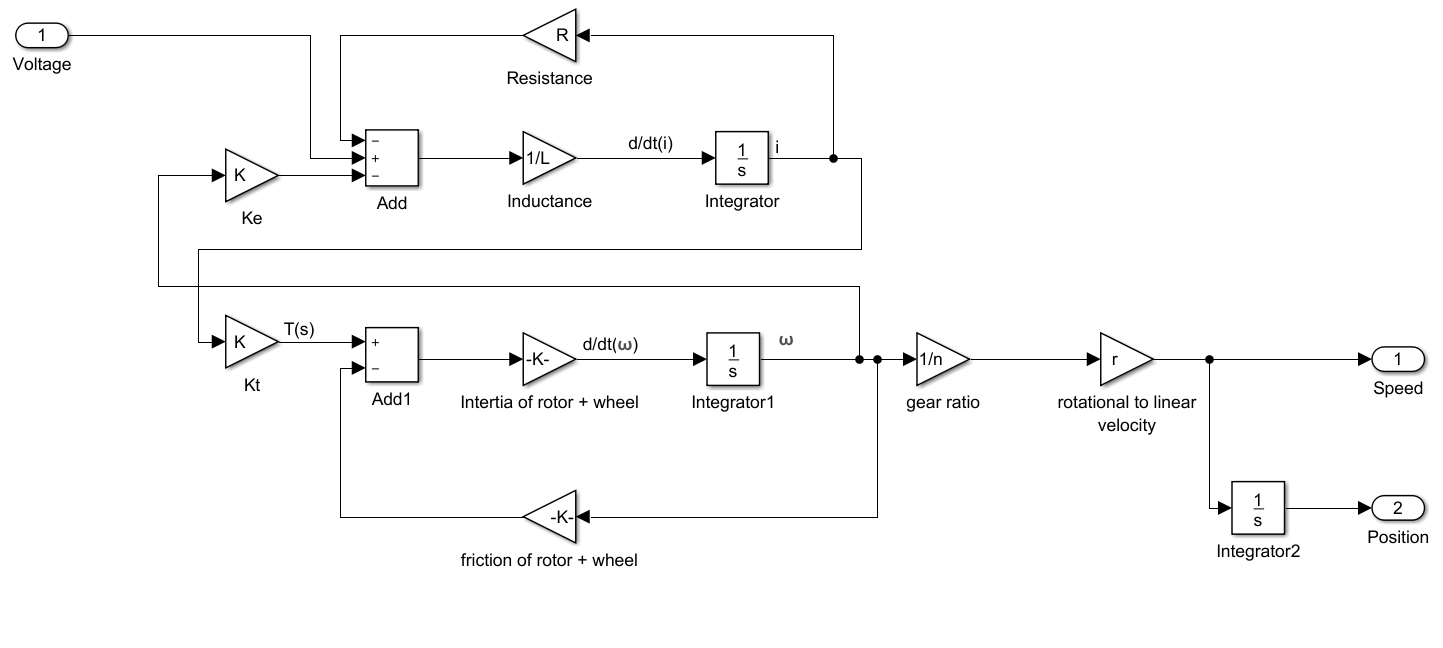
\includegraphics[width=1.1\textwidth]{dc_motorD}
\caption{DC Motor Block Diagram}
\label{fig::dcmfigure}
\end{figure}

The inclusion of the gear ratio (\textbf{n}) and the radius of the wheel (\textbf{r}) products to the angular velocity in the end of the block diagram, results in model scaling for the linear velocity (\textbf{v}) of the wheel. (\ref{eq12})

\begin{equation} \label{eq12}
v = r\omega
\end{equation}

Performing integration on the derived linear velocity results in obtaining the linear displacement of the wheels, later to be used with the kinematics model. 

To summarise, the goal was to relate the voltage to the speed. The input of the block diagram is the voltage of the motor (\textbf{V}) while the outputs are the linear speed caused by wheel rotation and the linear displacement, obtained from integrating the speed. The blocks comprising the upper and lower part of the block diagram, directly correspond to equation \ref{eq11} (upper part correspond to the electrical part of the motor; lower part correspond to the mechanical part of the motor).

Furthermore, as this paper is concerned with the development of a differential drive robot, the block diagram in figure \ref{fig::dcmfigure} is solely a subsystem of the complete kinematics model. That is, two DC motor subsystems are required in order to describe the complete motor/wheel dynamics. 


\subsection{Kinematics in simulink} 

Using equations \ref{eq13} and \ref{eq14} a simulink block diagram is constructed in figure \ref{fig::diff_simulink}.

\begin{figure}[h]
\centering
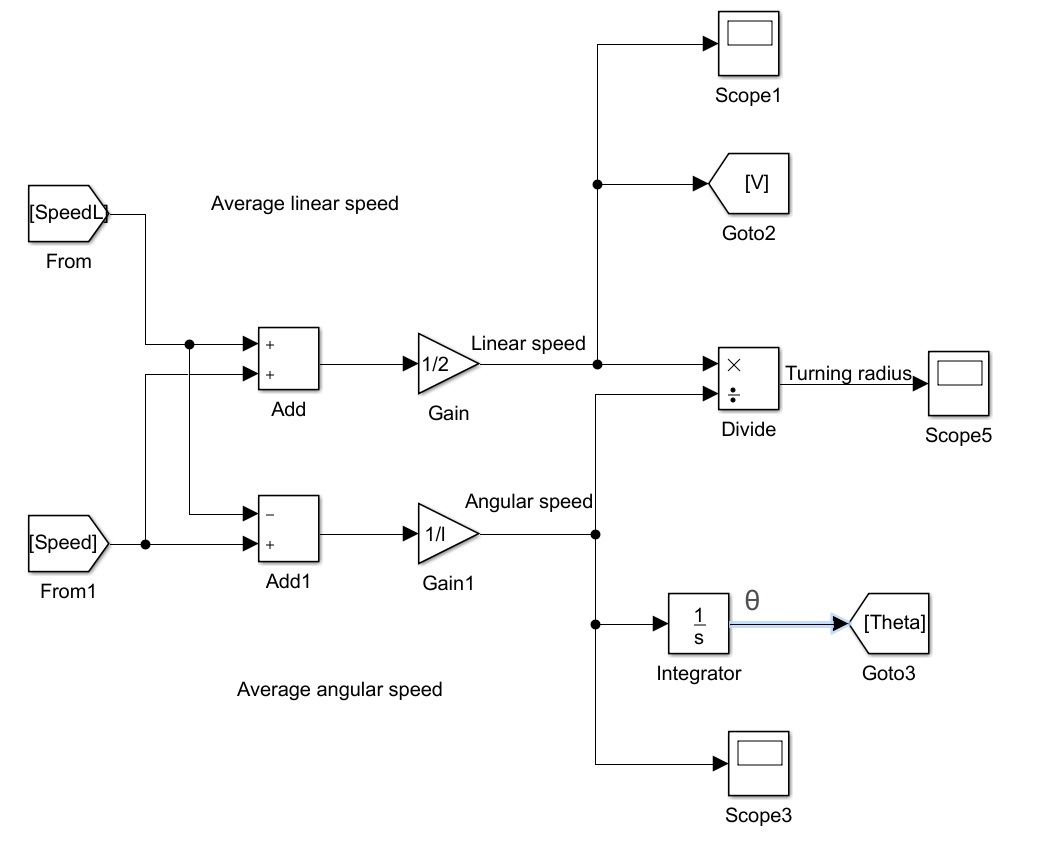
\includegraphics[width = 0.8\textwidth]{diff_drive_kin_simulink}
\caption{Differential drive kinematics}
\label{fig::diff_simulink}
\end{figure} 

The inputs are the individual wheel velocities, arranged to reflect the previously mentioned equations. The middle output is the turning radius \textbf{D}, which is governed by equation \ref{eq16}. The derived average linear speed is to be further used in equation \ref{eq20} to estimate the position of the robot based on it's angle through time, where the angle ($\theta$) is   obtain from integrating $\dot{\theta}$, which itself is the angular speed of the robot. 

\begin{figure}[h]
\centering
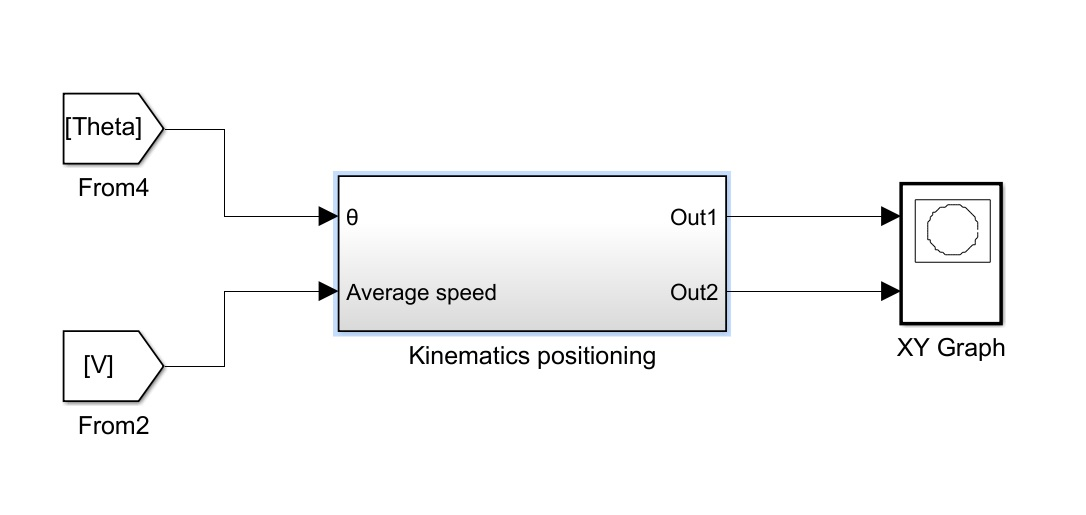
\includegraphics[width = 0.6\textwidth]{kin_pos_subsystem}
\caption{Positioning subsystem}
\label{fig::pos_sub}
\end{figure} 

In figure \ref{fig::pos_sub} the inputs are the the average speed and the orientation of the robot, while the outputs X and Y from equation \ref{eq20} are fed in a graph to observe the robot's trajectory through time. 

\begin{figure}[h]
\centering
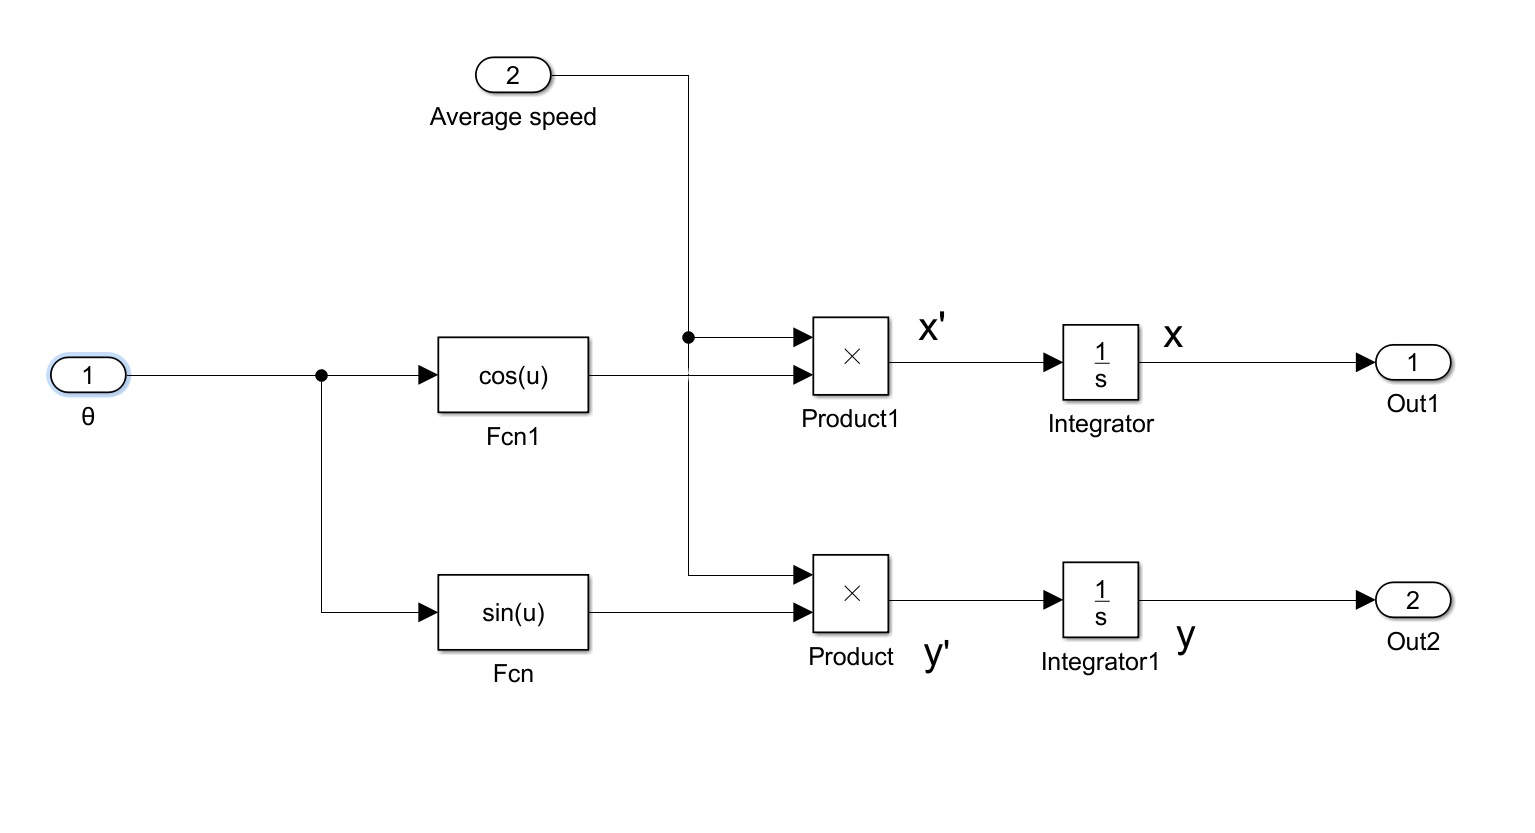
\includegraphics[width = 0.8\textwidth]{kin_model_pos}
\caption{Positioning subsystem}
\label{fig::pos_model}
\end{figure} 

The subsystem from figure \ref{fig::pos_model} is composed of blocks arranged to reflect equation \ref{eq20}. The outputs $\dot{x}$ and $\dot{y}$ are further integrated to graph the trajectory of the robot.

\section{Complete model}

In this section the complete system model is derived. It includes motor dynamics and robot kinematics. That is, the behaviour of the robot is analysed and compared with the expected performance.

\begin{figure}[h]
\centering
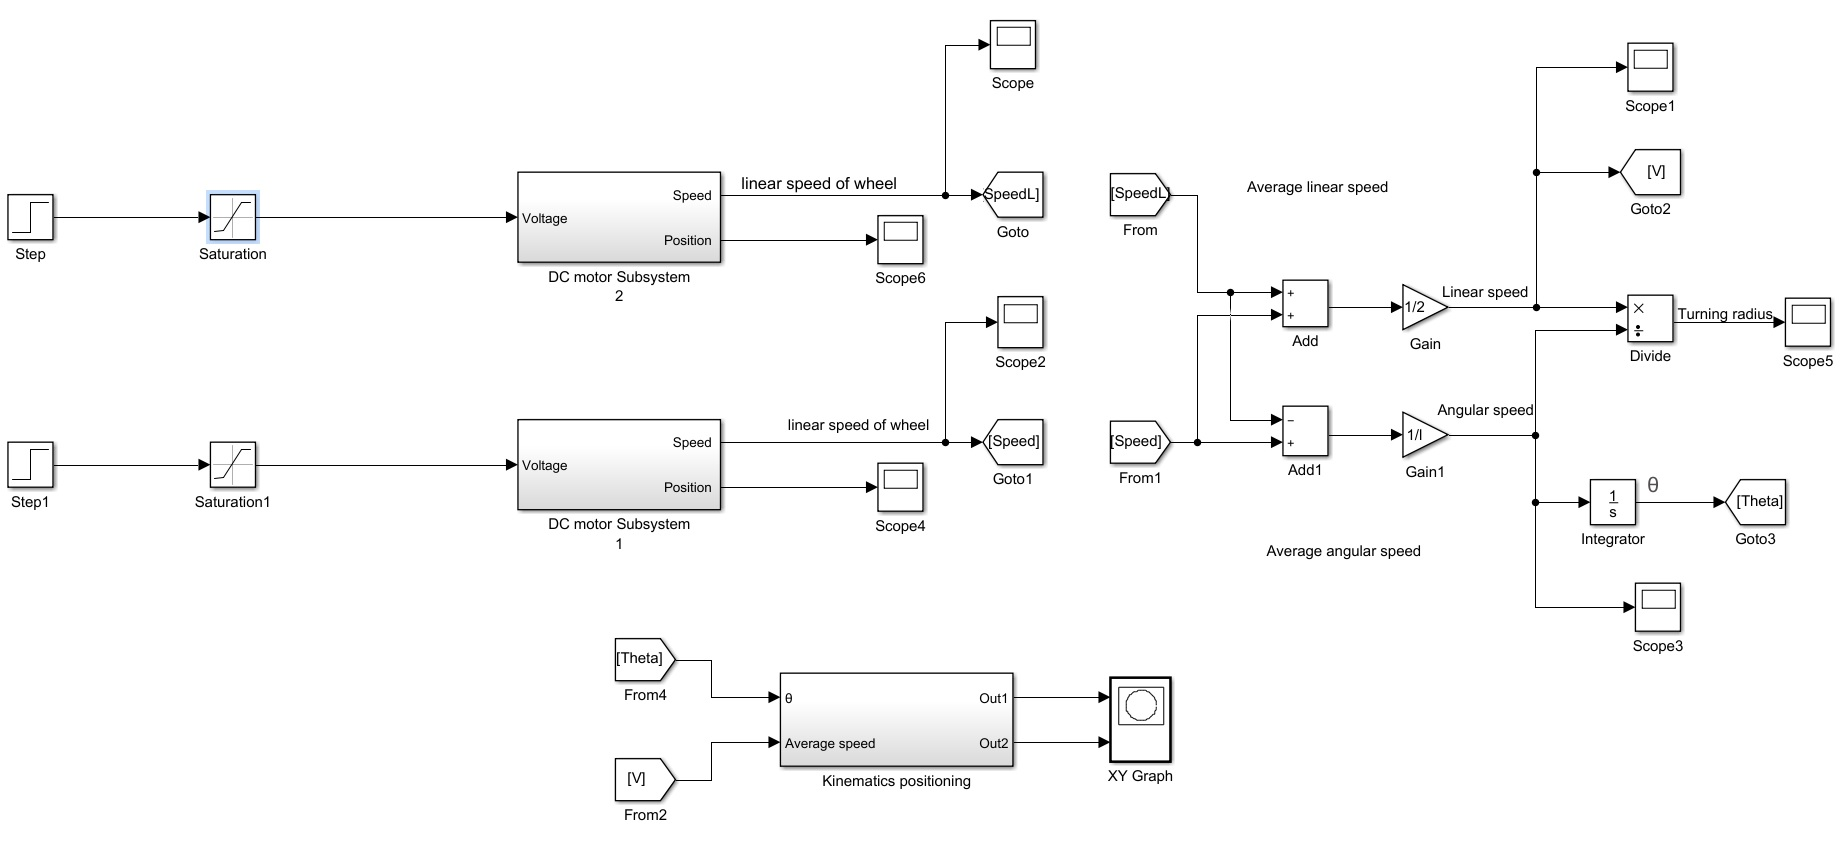
\includegraphics[width = 0.8\textwidth]{comp_model_simulink}
\caption{Complete system model}
\label{fig::com_model}
\end{figure} 

In figure \ref{fig::com_model}, the complete system model for a differential drive robot could be observed. As previously mentioned, a differential drive consist of two DC motors, thus to accurately model the relations, two motor subsystem as described in section \ref{dc_model}, are used. 

\subsection{DC motors model analysis} 

The two DC motors are in the top left corner of the model in figure \ref{fig::com_model}. A step function block is used to simulate the voltage applied to the motor, alongside a saturation block that limits the model from  computing with values greater than the maximum allowed voltage in the physical motor. 

The motor model proposed in section \ref{dc_model} is constructed using only linear blocks, thus the open-loop response could be observed by providing a unit step input and observing the response through a scope block. 

\begin{figure}[h]
\centering
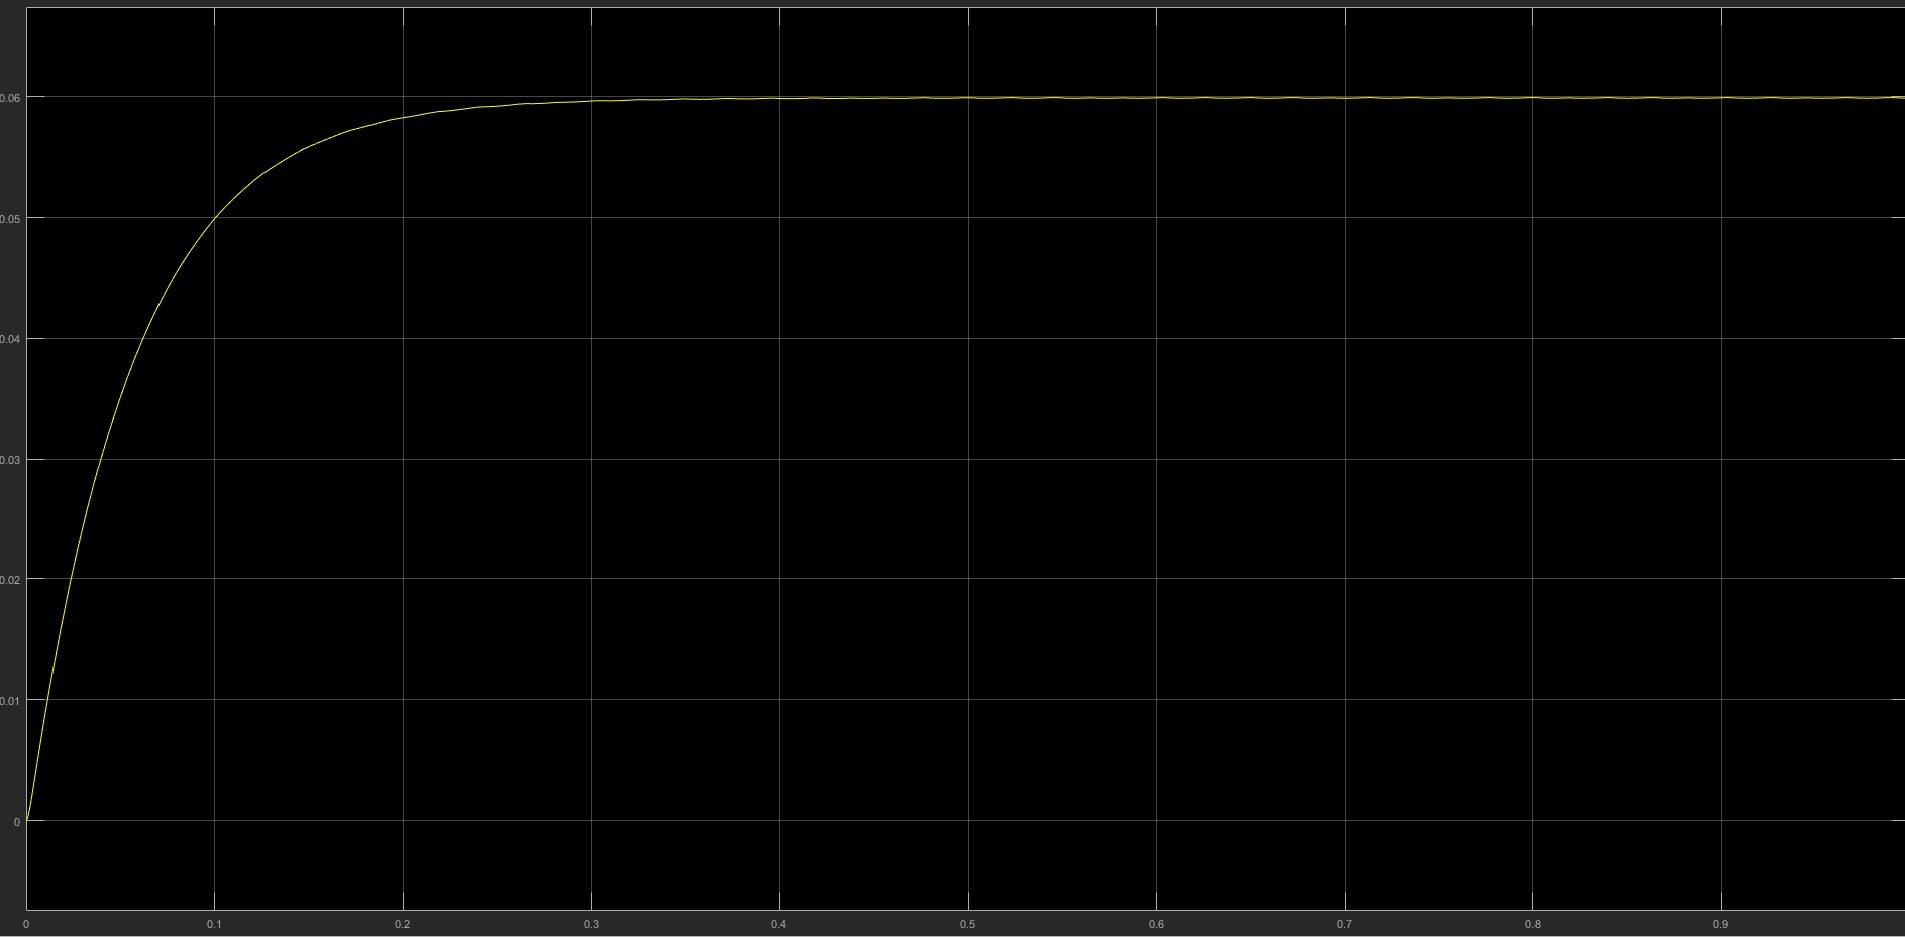
\includegraphics[width = 0.7\textwidth]{motor_openl_step}
\caption{Step response of DC motor}
\label{fig::dc_step}
\end{figure} 

Figure \ref{fig::dc_step} is consistent with the expected step response of a DC motor. When 1 Volts is applied as a step input, the motor achieves maximum speed of 0.06 cm/s (after conversion to linear speed) However to further understand the results, linear analysis on the subsystem has been performed.

\begin{figure}[h]
\centering
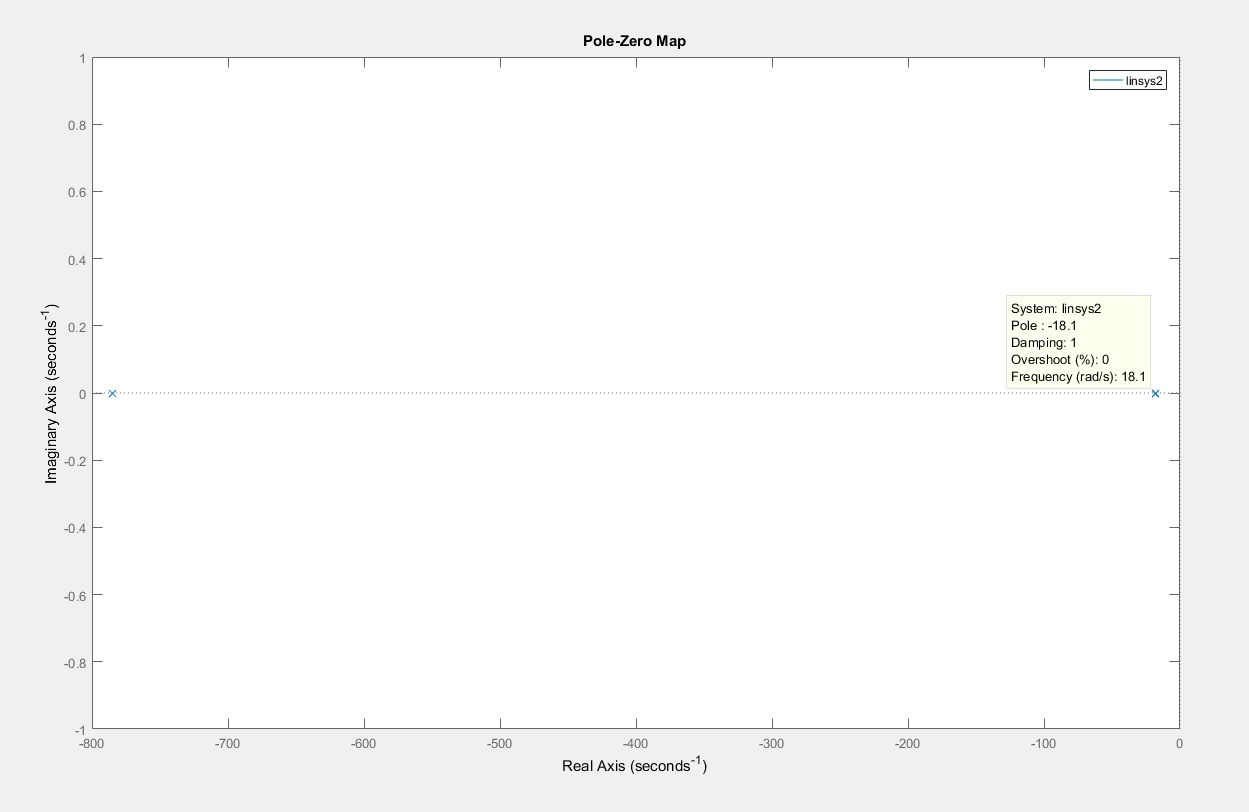
\includegraphics[width = 0.7\textwidth]{Pzmap_dc}
\caption{Pole-Zero map of DC motor}
\label{fig::dc_pz}
\end{figure} 

From figure \ref{fig::dc_pz}, it is clear that the open-loop subsystem has two real poles in the left hand plane. That is ,no oscillations or overshoot present as it could be seen in the step response. Furthermore, the slower of the two poles will dominate the dynamics of the system, prompting the system to behave as it was first-order. 

Obviously, both motors' models behave the same while applying the same step input. Nevertheless, it is important to understand that in real life this may not be the case, as the constants used in the model may not reflect accurately both real-life counterparts.

\subsection{Kinematics model analysis} \label{kin_analysis}

We discussed in subsection \ref{kin_model} how small fluctuation in the speed of each motor, will results in a change of the trajectory of the whole robot. It is important to verify that the cases laid in the above mentioned subsection hold true.

\begin{figure}[h]
    \centering
    \begin{subfigure}[h]{0.47\textwidth}
        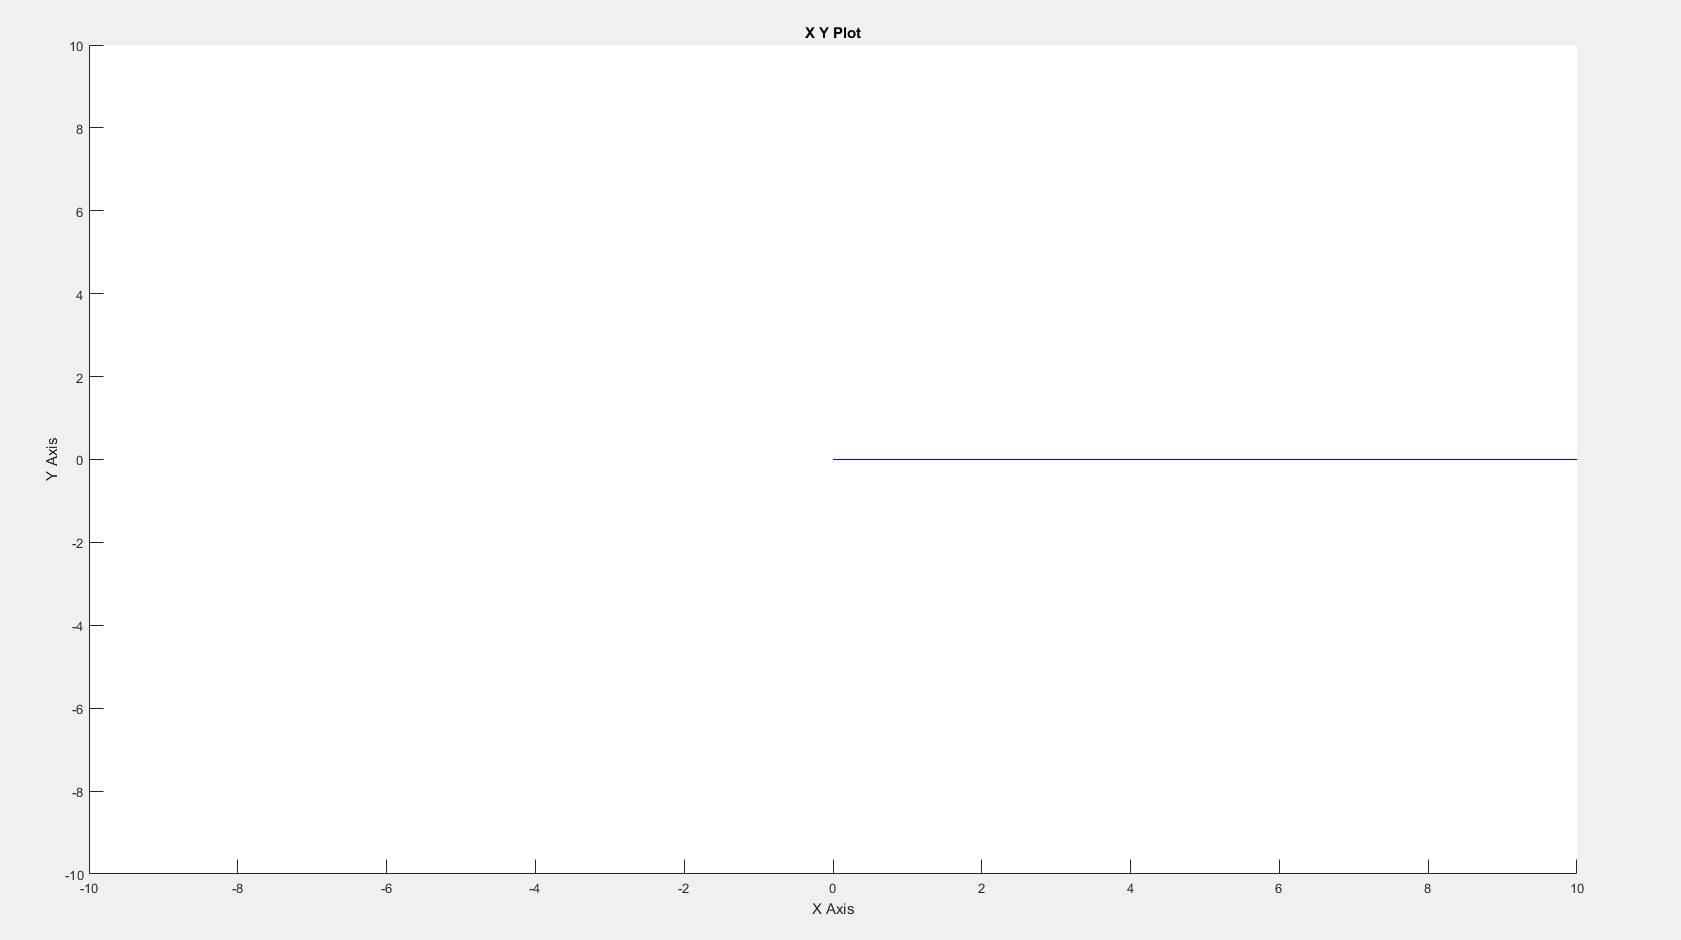
\includegraphics[width=\textwidth]{x_y_equalV}
        \caption{XY-graph}
        \label{fig:v_l=v_r}
    \end{subfigure}
    ~ %add desired spacing between images, e. g. ~, \quad, \qquad, \hfill etc. 
      %(or a blank line to force the subfigure onto a new line)
    \begin{subfigure}[h]{0.47\textwidth}
        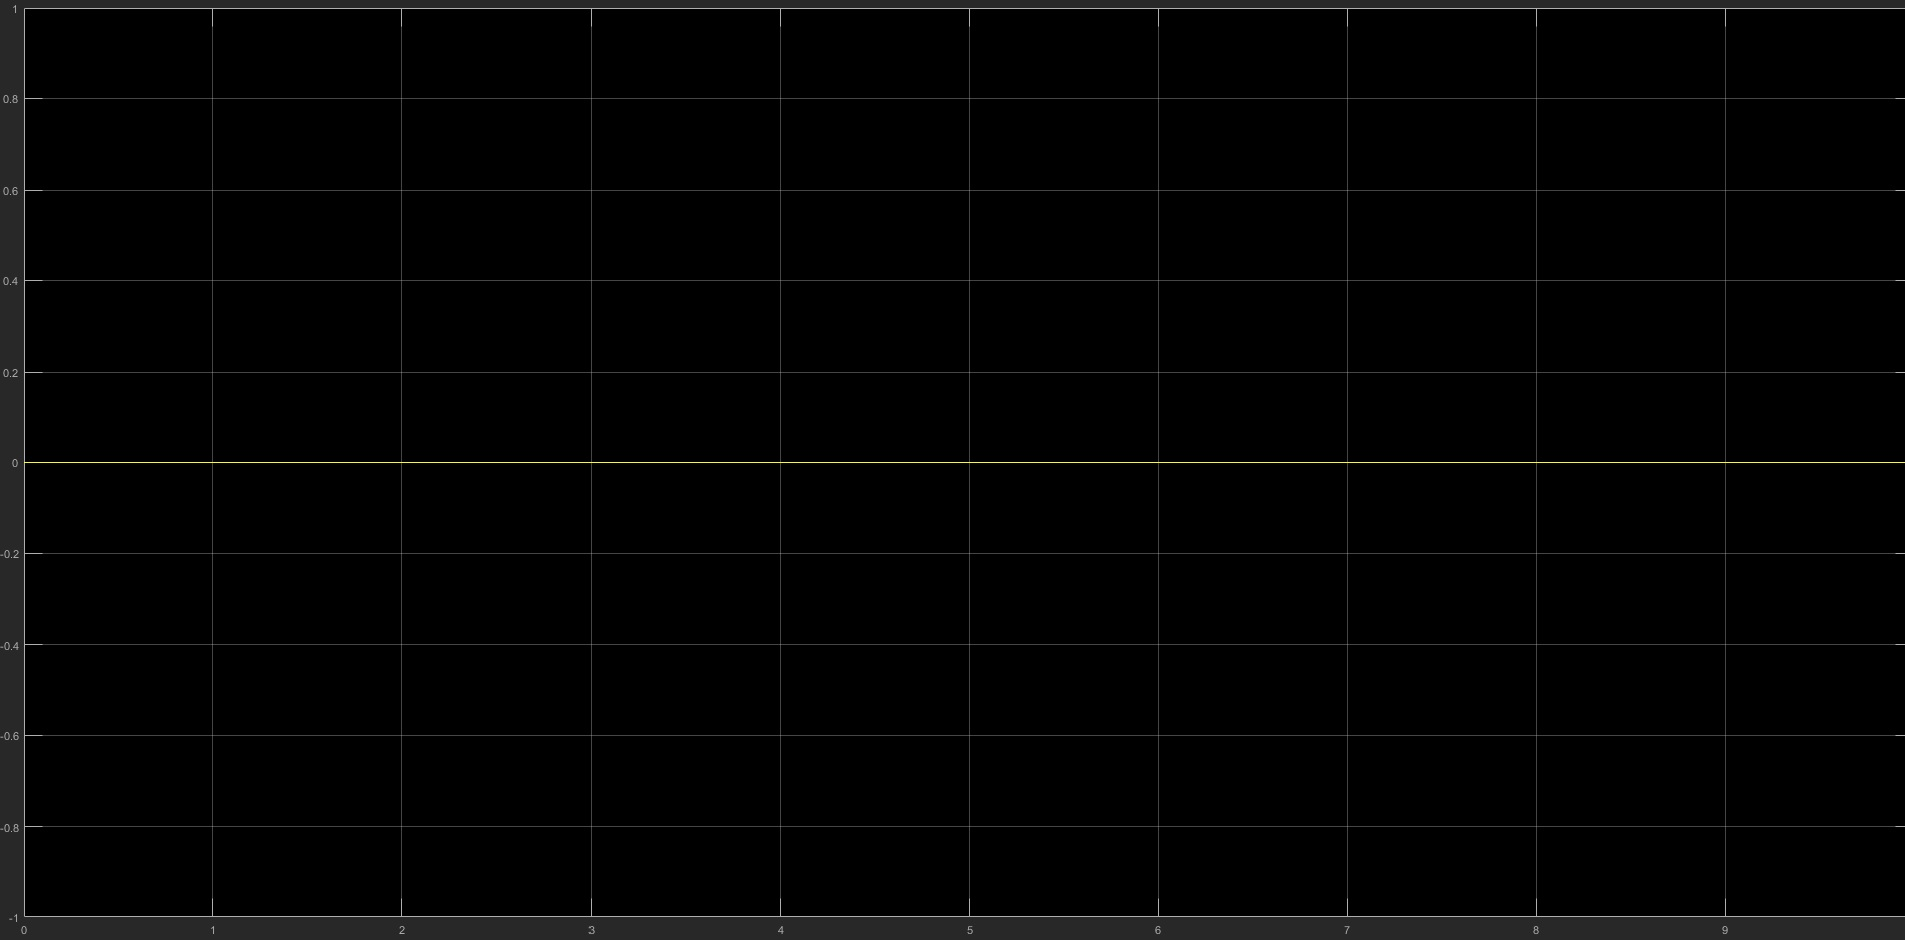
\includegraphics[width=\textwidth]{AS_equalV}
        \caption{Turning speed}
        \label{fig:Wv_l=v_r}
    \end{subfigure}
    ~ %add desired spacing between images, e. g. ~, \quad, \qquad, \hfill etc. 
    %(or a blank line to force the subfigure onto a new line)
    \caption{For equal velocities}\label{fig:eqV}
\end{figure}

In figure \ref{fig:v_l=v_r}, when both wheel velocities match ($\boldsymbol{v_r = v_l}$), the trajectory the robot partakes is a straight line. 

As to be expected, the turning speed in figure \ref{fig:Wv_l=v_r} remains zero for as long as the velocities of each wheel match.

\newpage

The other case scenario is when one of the wheels has zero velocity (the other wheel's velocity can not be equal to zero).

\begin{figure}[h]
\centering
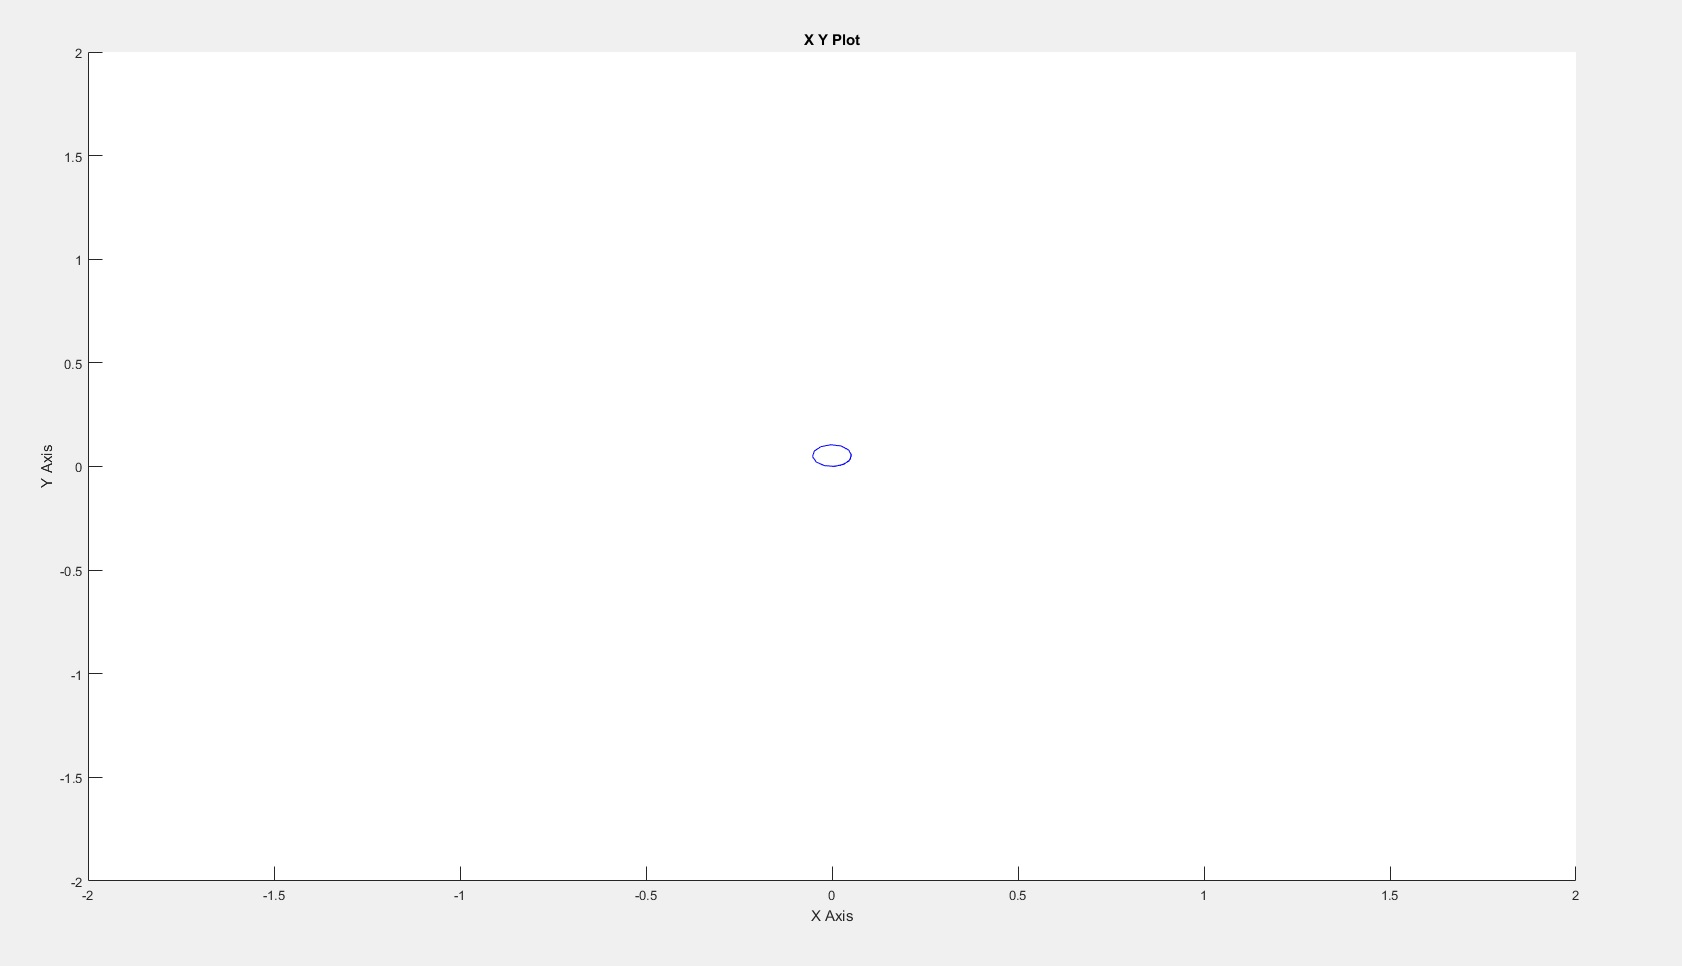
\includegraphics[width = 0.7\textwidth]{x_y_zeroV}
\caption{XY-graph for zero velocity left wheel}
\label{fig::ZeroV}
\end{figure} 

The expected behaviour is rotation where the ICC is positioned at the zero velocity wheel. Furthermore, the turning speed should be constant, while the turning radius equal to $\frac{l}{2}$.

\begin{figure}[h]
    \centering
    \begin{subfigure}[h]{0.47\textwidth}
        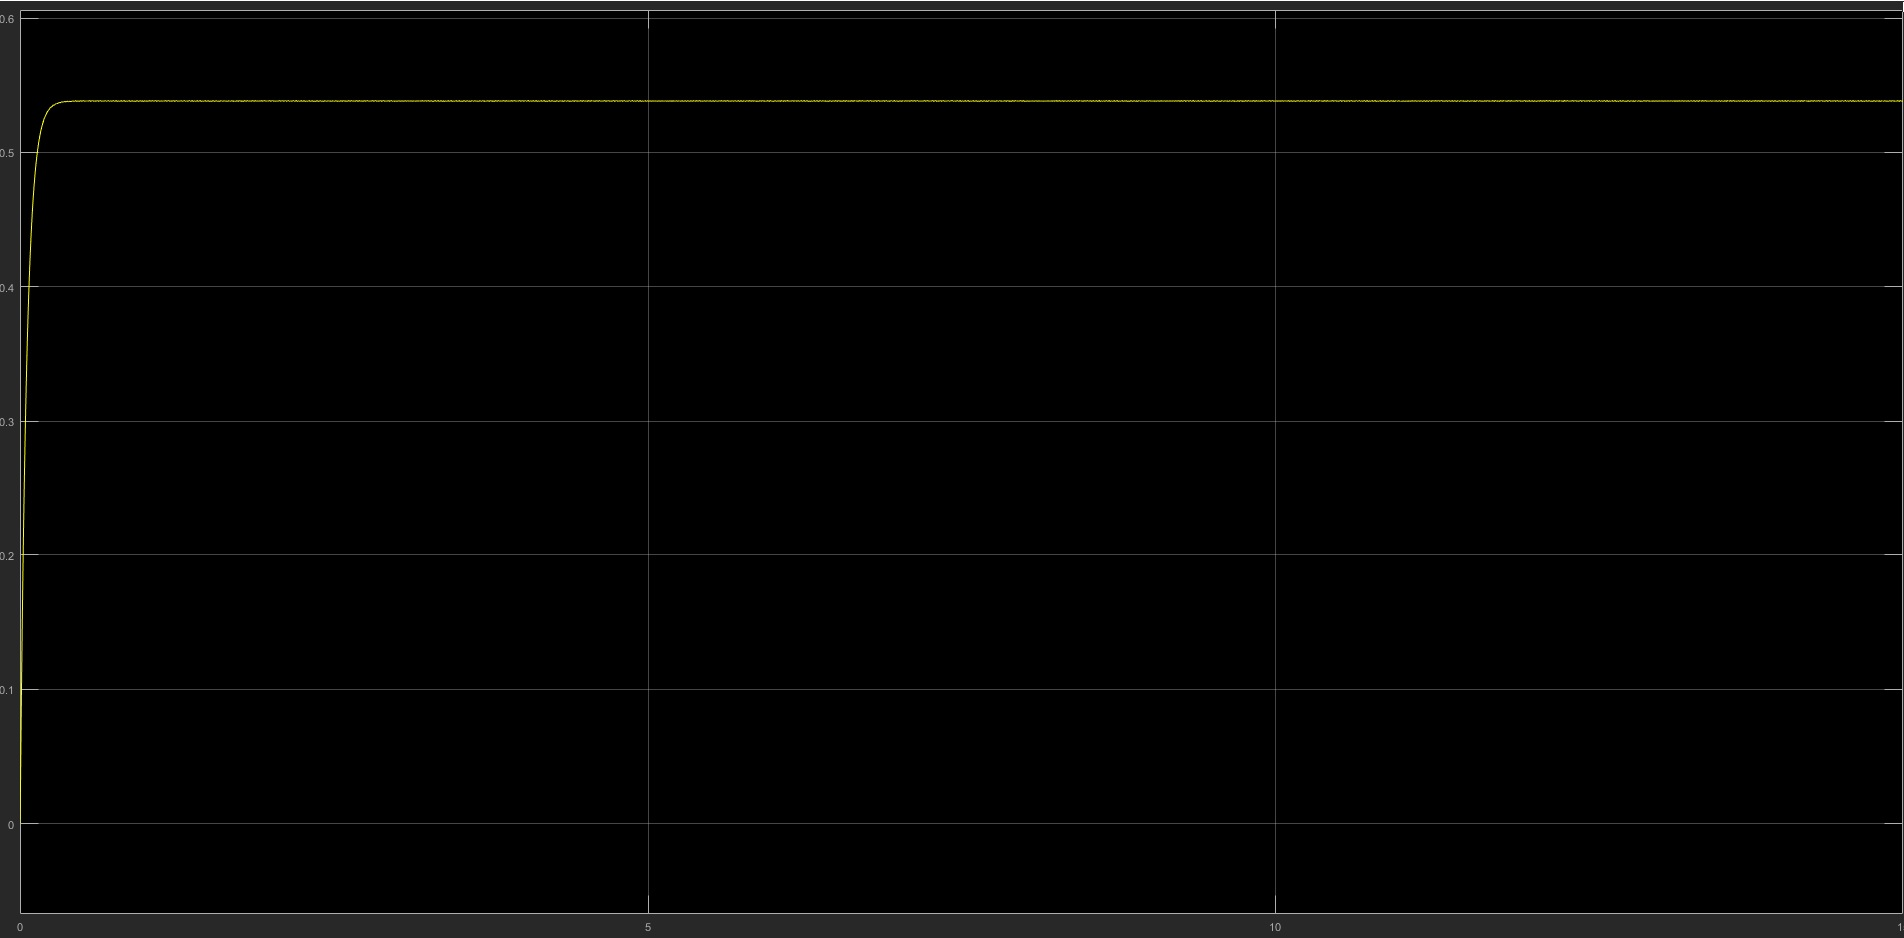
\includegraphics[width=\textwidth]{turning_speed_zeroV}
        \caption{Turning speed}
        \label{fig:TzeroV}
    \end{subfigure}
    ~ %add desired spacing between images, e. g. ~, \quad, \qquad, \hfill etc. 
      %(or a blank line to force the subfigure onto a new line)
    \begin{subfigure}[h]{0.47\textwidth}
        \includegraphics[width=\textwidth]{turning_rad_zeroV}
        \caption{Turning radius}
        \label{fig:RzeroV}
    \end{subfigure}
    ~ %add desired spacing between images, e. g. ~, \quad, \qquad, \hfill etc. 
    %(or a blank line to force the subfigure onto a new line)
    \caption{For zero velocity left wheel}\label{fig:zeroV}
\end{figure}

In figure \ref{fig:TzeroV} it takes 1.5 seconds to reach constant turning speed, while in figure \ref{fig:RzeroV}, the turning radius is exactly 0.052 cm, which is exactly half of the distance between wheels. This satisfies the expected behaviour. \\


However to truly picture why necessary control needs to be applied in order to maintain constant speed for both wheels, a simulation was performed where the inputs of the step function differ only by 0.1 V. That is, $\boldsymbol{v_r \approx v_l}$. 

In figure \ref{fig:approxV} we can clearly see that the trajectory the robot partakes is similar to an arc. That is, even small fluctuation in the speed of one motor, will result in a circular motion with albeit a relatively large turning radius (\ref{fig:RapproxV}. 

\newpage

\begin{figure}[h]
    \centering
    \begin{subfigure}[h]{0.47\textwidth}
        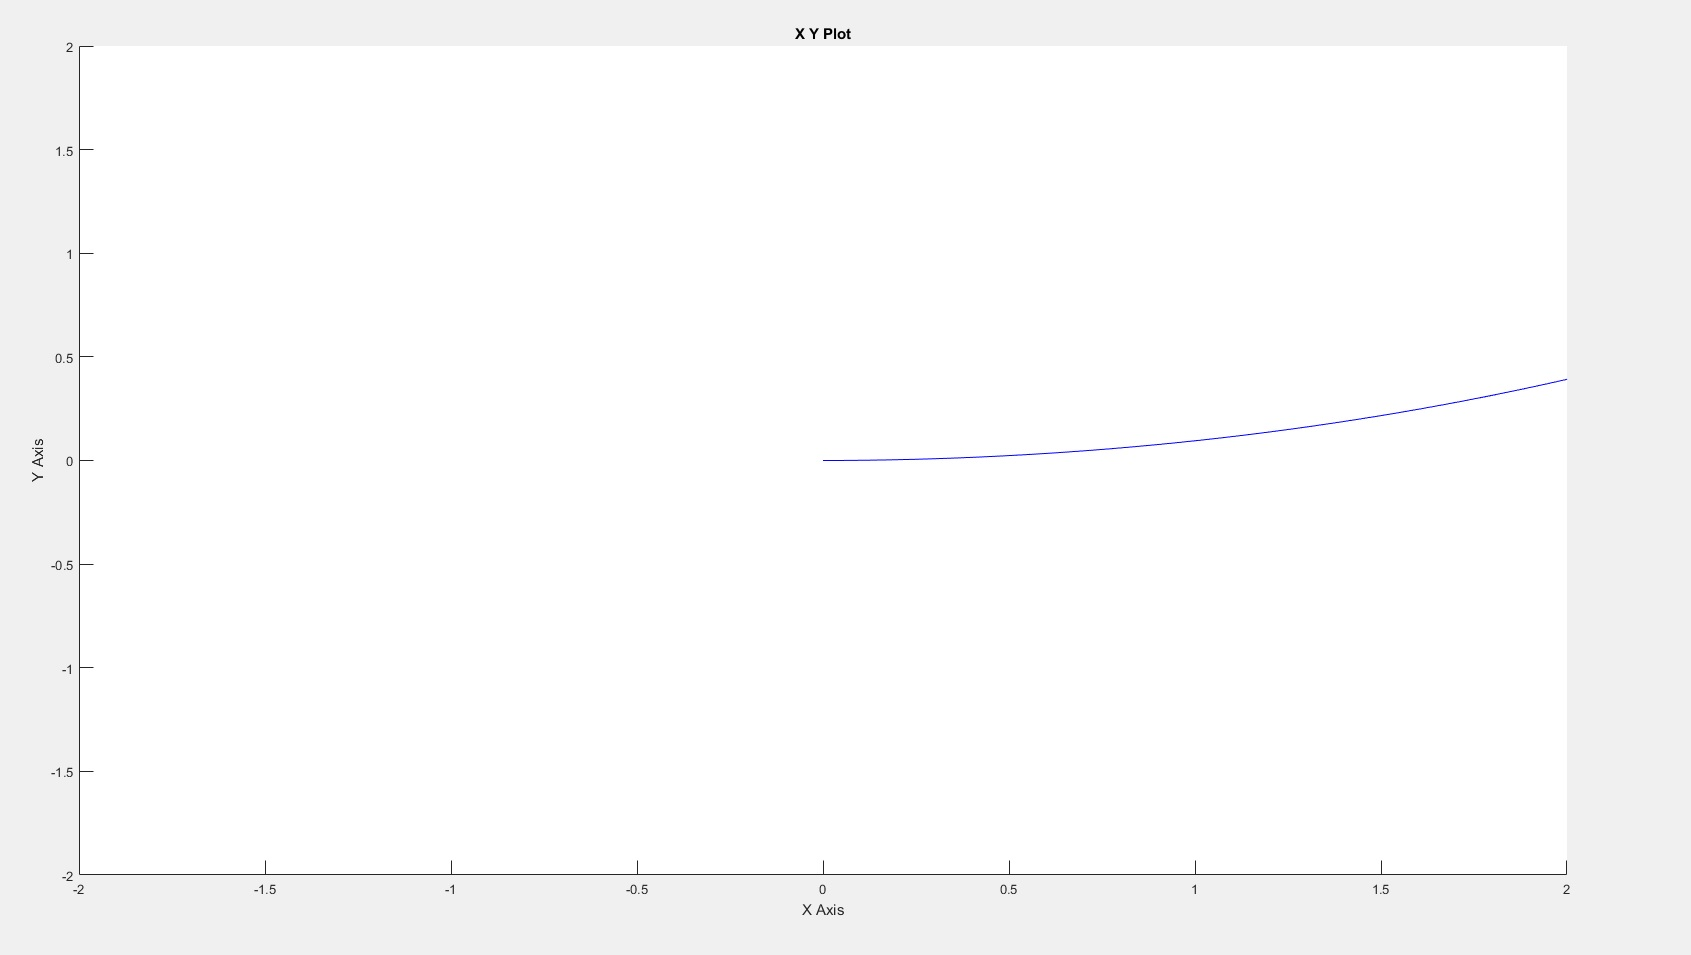
\includegraphics[width=\textwidth]{XY_approxV}
        \caption{XY-graph}
        \label{fig:approxV}
    \end{subfigure}
    ~ %add desired spacing between images, e. g. ~, \quad, \qquad, \hfill etc. 
      %(or a blank line to force the subfigure onto a new line)
    \begin{subfigure}[h]{0.47\textwidth}
        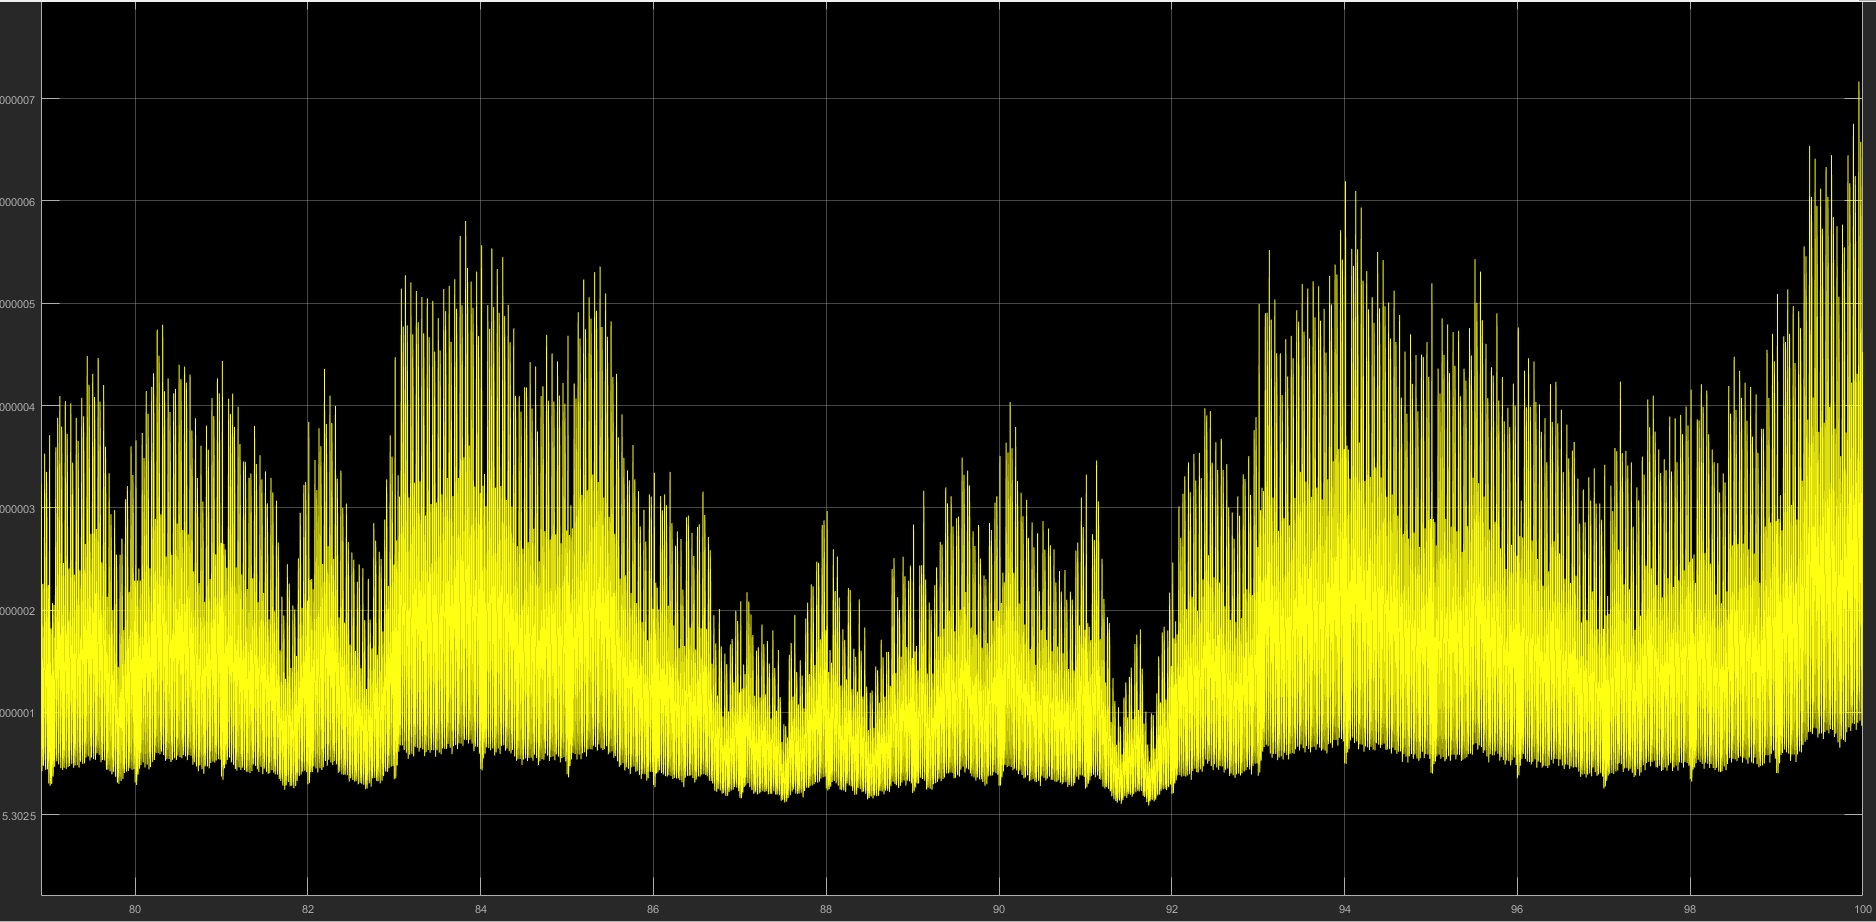
\includegraphics[width=\textwidth]{R_approxV}
        \caption{Turning radius}
        \label{fig:RapproxV}
    \end{subfigure}
    ~ %add desired spacing between images, e. g. ~, \quad, \qquad, \hfill etc. 
    %(or a blank line to force the subfigure onto a new line)
    \caption{For different velocities}\label{fig:approxV}
\end{figure}

Clearly, a controller is necessary to maintain constant speed in both wheel, when the robot is required to follow a linear trajectory.

\section{Cruise Control}

In this section, the problem of necessary control is addressed. 

\subsection{PID controller}

As it was previously discussed, small fluctuation in the individual speeds of the wheels would cause distortion in the linear movements. Differential drive robots are a perfect example of the necessity of a control algorithm.

First of all, it needs to be mentioned that in a real life scenarios, several tools would be used in order to provide basic navigation. The simplest way to limit the motor's speed to a certain percentage would be to use Pulse Width Modulation (PWM). Nevertheless, it would remain an open loop system, that is, no information would be provided to verify that the individual speeds of  the wheels match. In order to create a closed loop system, some feedback is needed. The most common way would be with an encoder. This way, the individuals speed of each wheel could be compared and theoretically adjusted. 
Proportional integral derivative (PID) controller is potential solution. In a differential drive robot, the idea would be to have a PID controller for both motors and feedback from the encoders. For example, if the goal is to maintain constant speed (which would ensure linear movement), a setpoint value would be needed, as well as constant feedback from the encoders. The two values would be compared and an error value will be generated:\cite{PID}

\begin{equation}
error = setpoint - encoder\,reading
\end{equation}

The error value would be used to calculate the amount of alterations required on the motor speed to reduce the error to a theoretical zero. That is, a plain Proportional controller, would feed the error value to the PWM output after multiplying it by the proportional gain constant. 

\begin{equation}
C = eK_p 
\end{equation}

Where C is the control variable, e is the error and $K_p$ the proportional gain. 
However, if a large $K_p$ value is used, it may cause overshoot followed by oscillations that would result in potential jittering as robot's behaviour. This could be solved by using a PD controller, where the rate of the change of the error is taken into account as well ($\frac{de}{dt}$). 

\begin{equation}
C = eK_p + \frac{de}{dt}K_d
\end{equation}

Where $K_d$ is the derivative gain. 
In general a PD controller might be sufficient enough to maintain constant speed in the motor, nevertheless adding an Integral control could improve steady state performance by integrating all previous errors and detect accumulating errors. Last the complete equation of a PID controller:

\begin{equation}
C = eK_p + K_i\int_{0}^{t} e \,dt + \frac{de}{dt}K_d
\end{equation} 

\subsection{Simulink Closed-loop Response} 

Understanding how a PID controller could potentially remove fluctuations in the motors' speed, was necessary to apply it to the motors model from section \ref{dc_model}. 

\begin{figure}[h]
\centering
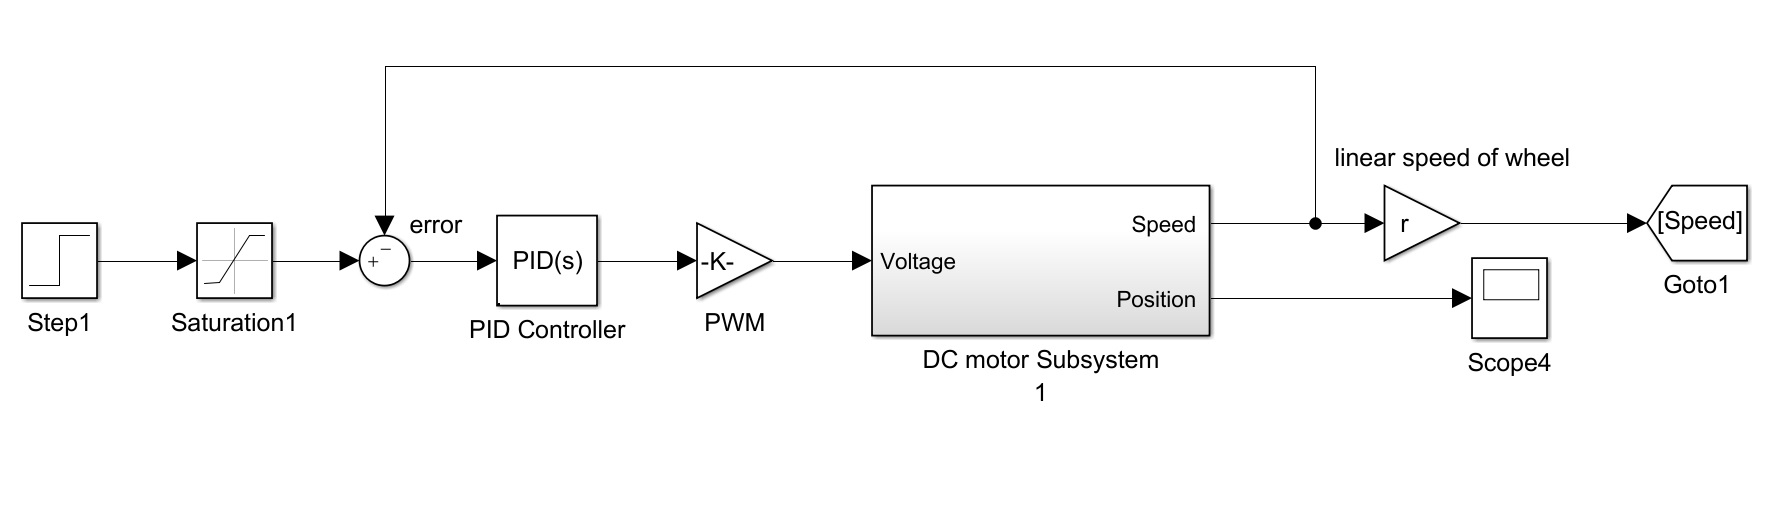
\includegraphics[width = 0.9\textwidth]{PID_motor}
\caption{Closed-loop motor subsystem}
\label{fig::PID_motor}
\end{figure}

In figure \ref{fig::PID_motor}, the closed-loop control system is shown. The system consist of a PID controller, a gain block to represent the PWM output (in percentage), and a negative feedback from the angular speed of the motor (represented by an encoder in real life). 

\begin{figure}[h]
\centering
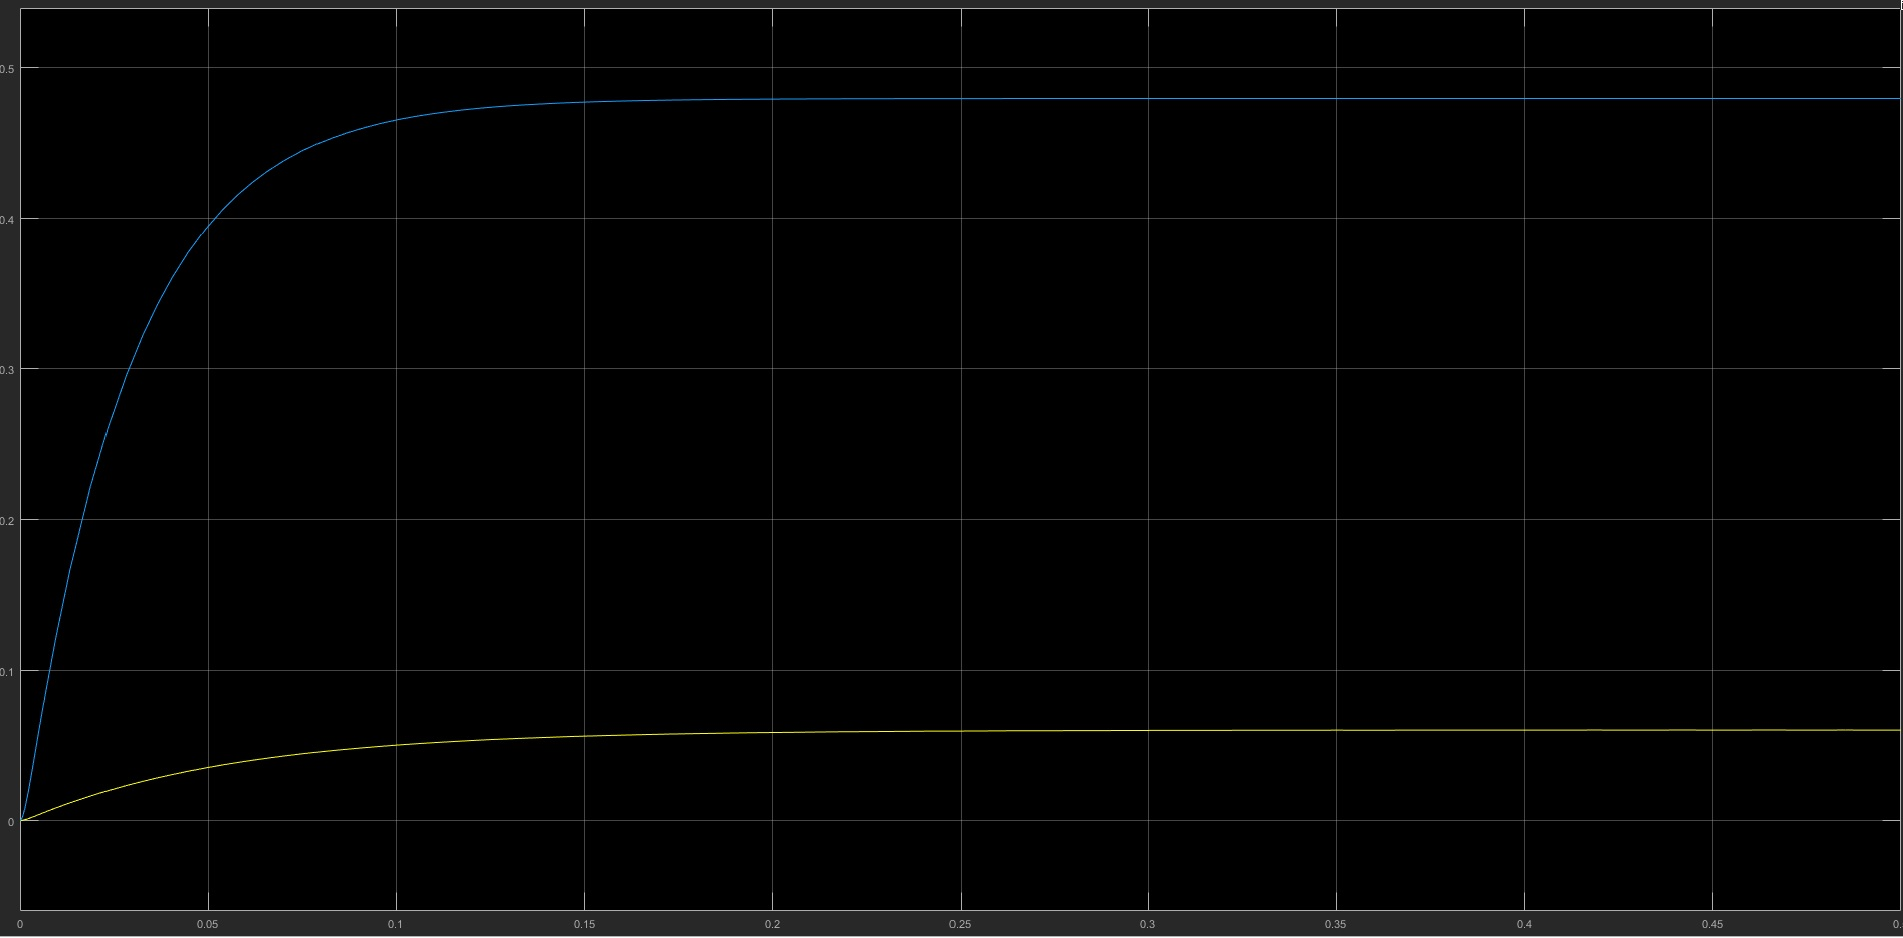
\includegraphics[width = 0.7\textwidth]{CL_OL_comp}
\caption{Comparison between open-loop and closed-loop step response}
\label{fig::PID_comp}
\end{figure}

In figure \ref{fig::PID_comp}, the yellow curve represents the open-loop step response, while the blue curve the closed-loop step response. The final value in the step function is set to 1, and it is obvious that steady state error is quite large in the open-loop case and lower but not gone in the close-loop case. Thus to further adjust the PID values, a set of design criteria had to be met.

\begin{itemize}
\item Settling time < 1 sec
\item Overshoot < 5 \%
\item Steady-state error < 1\%
\end{itemize} 

Using Matlab PID tuner, the design criteria are met when the values correspond to those in figure \ref{fig::PID_tuner}.

\begin{figure}[h]
\centering
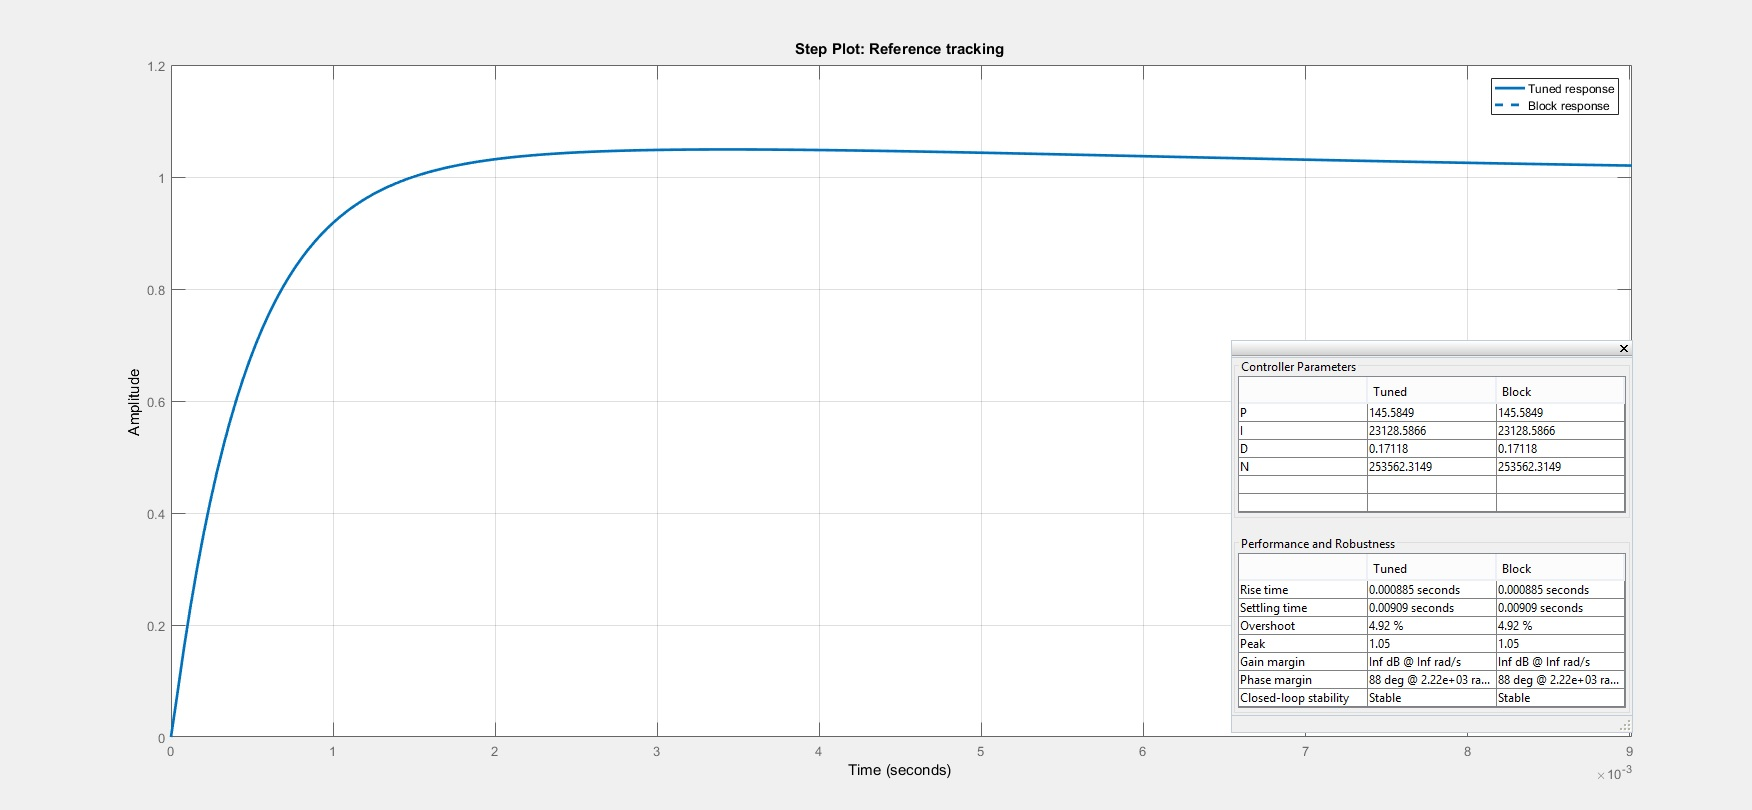
\includegraphics[width = 0.7\textwidth]{PID_tuner}
\caption{Matlab PID tuner and gains adjustment}
\label{fig::PID_tuner}
\end{figure}

Although the tuned values cover the design criteria, a more practical approach such as Ziegler–Nichols method has to applied when designing a controller for the physical robot system. 